% Acceleo M2T
\subsection{Acceleo}
\label{acceleo}
Acceleo is an open source Code generator that allows the creation of code starting from any kind of text which structure is described by a meta-model. Acceleo was released in its first GNU public license in 2006 and later joined the Eclipse Foundation universe going through several major modifications to comply with the MOFM2T specifications. As today, Acceleo version 3.3 is available as a free plugin for the Eclipse development environment. Figure \ref{fig:AcceleoScenario} represents the classic Acceleo usage scenario where a model (and its meta-model) together with a target module (Java, Php, etc.) are provided as input to the generator which outputs the files written in the target language.

\begin{figure}
  \begin{center}
    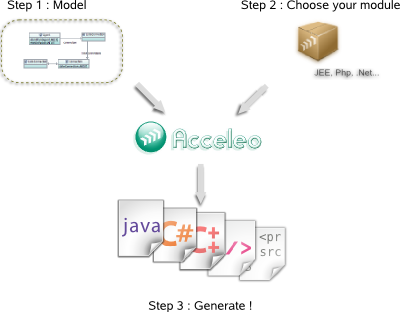
\includegraphics[scale=0.9]{pictures/Acceleo-scenario-en.png}
    \caption{Acceleo usage scenario \cite{AcceleoPresentation}. A model and its module (Java, Php, etc.) are given as input to the Acceleo Generator which gives in output the files generated in the target language.}
    \label{fig:AcceleoScenario}
  \end{center}
\end{figure}

\paragraph{An Acceleo example}
Acceleo is a template-based model-to-text transformation (see Section \ref{m2m&m2t}), where the user manually writes the static part of his code and fills the (dynamic) code that changes with Acceleo parameterized snippets.
For example, let's imagine a transformation from an input file written in the BPEL language to a Java file. As shown in Listing \ref{lst:AcceleoGettersExample}, we can see how Acceleo creates a generic template to generate Java getters methods for the private attributes of a class. Passing to the Acceleo function a list of Variables (varNameList), it goes through it and for each variable it creates a public method named \textit{get} + \textit{name} of the variable with first letter capitalized with return-type the type of the variable. This proves very useful when the list of variables is huge and dynamic, making a manual procedure a too cumbersome and error-prone task.

\begin{workflow-code}{Acceleo creating the Java getters for a list of variables. The code out of square brackets is static code}{lst:AcceleoGettersExample}
[for (aVar : Variable | varNameList )]
public [aVar.Type.toUpperFirst()/] get[aVar.name.toUpperFirst()/]() {
	return [aVar.name.toLowerFirst()/];
}
\end{workflow-code}

\subsubsection{How the parameterization in Acceleo works}
\label{AcceleoParametirazion}
The snippets of code included in square brackets in Figure \ref{lst:AcceleoGettersExample} are Acceleo code parameterized using the BPEL meta-model, where a BPEL file is used as input. As the structure of the BPEL language is well defined in an ecore schema published by the Eclipse Foundation (see Section \ref{metamodelExample}), we always know that once we encounter a \textit{Variable} element, it must have a BPEL \textit{name}, a BPEL \textit{type}, etc. 
Thus, Acceleo permits us to search into the file for the elements (parameters) we need, take out the attributes and generate the corresponding output code.
The mechanism to look for specific elements in a file used by Acceleo is a superset of the Object Constraint Language (OCL) \cite{UML20OCL}. OCL is a declarative language that describes rules applying to UML (and its dialects) models. With OCL it is possible to apply constraints as well as query a model; it is mainly used to specify expressions that cannot be represented on a model by visual or diagrammatic notations.

\subsubsection{Acceleo Architecture}
\label{AcceleoArchitecture}
Figure \ref{AcceleoArchitecture} depicts the overall 3-part architecture of the Acceleo generator, described in the next three paragraphs.
\paragraph{Modeler}
On the left, there is represented the modeling side, where models are created and given as inputs to the generator. As far as the model is well defined and has a meta-model descriptor, any kind of model can be used: UML, XMI, XML, some other programming languages or a custom created model. One thing to note is that models are created outside of the Acceleo framework. Generally, one would want to use preexistent models (e.g. the UML model of an existent application) that will generate through Acceleo code written in a target language (e.g. Java). 
An example of Modeling tools completely compatible in terms of standards with Acceleo, is the Eclipse Modeling Framework (see Section \ref{EMF}).   
\paragraph{Eclipse Acceleo Plugin}
In the middle there stands the Acceleo generator. Acceleo reuses the native Eclipse components regarding model transformations and code generation. For example, Acceleo reuses the Java Emitter Templates (JET) technology, which is a Model-to-Text generator aimed at Java output.
\paragraph{Generation}
On the right, there are represented the output modules one can obtain through an Acceleo generation. Virtually any language is supported, and documentation can be generated as well.

\begin{figure}
  \begin{center}
    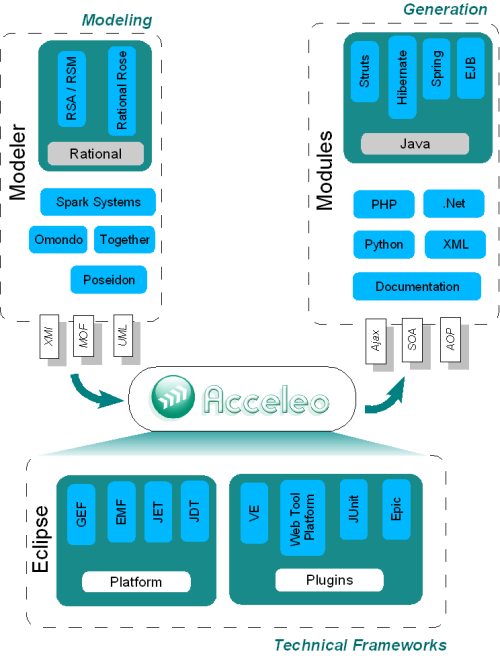
\includegraphics[scale=0.7]{pictures/acceleo-archi-en.png}
    \caption{Architecture of the Acceleo Generator \cite{AcceleoArchitectureWeb}. Models are created and given as input to the generator which reusing the Eclipse text generation technologies outputs the target module}
    \label{fig:AcceleoArchitecture}
  \end{center}
\end{figure}





